\documentclass[12pt]{article}
\usepackage{tabularx, makecell, multirow, ctex, graphicx, abstract, booktabs, amsmath}

\begin{document}
	
	\title{美赛自用攻略——论文手}
	\author{YAN}
	\maketitle
	
	\begin{abstract}
		
		美赛中摘要部分是最重要的,其次是正文。
		
	\end{abstract}
	
	\section{摘要}
		\subsection{美赛论文模板与写作方法}
			\begin{figure}[htbp]
				\centering
				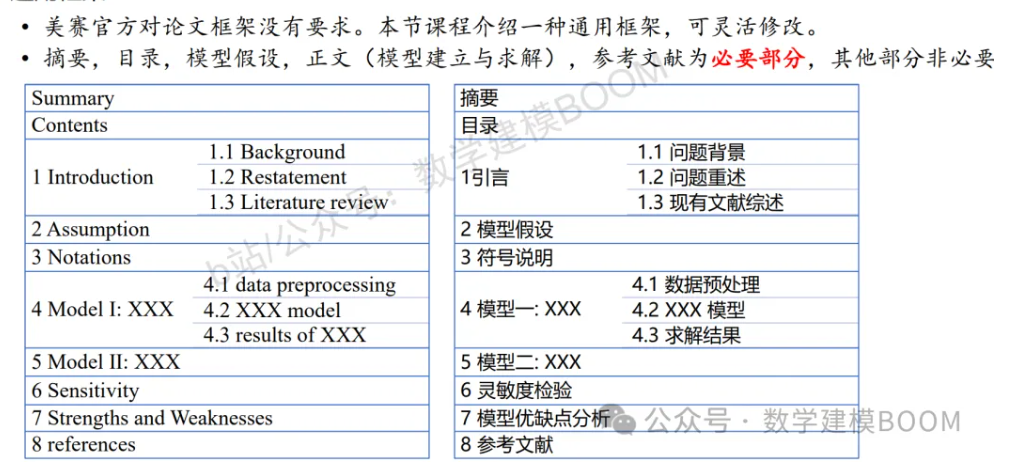
\includegraphics[width=1\textwidth]{1}
				\caption{美赛论文模板与写作方法}
				\label{fig:1}
			\end{figure}
		\subsection{比赛规则对论文的要求}
			\begin{itemize}
				\item[$\bullet$] 在第一页摘要页左上角写选择的问题,A-F之一
				\item[$\bullet$] 右上角写队伍号
				\item[$\bullet$] 论文中不得出现任何姓名和学校等信息
				\item[$\bullet$] 提交的文件为pdf格式,文件名为队伍号
				\item[$\bullet$] 文件必须小于20MB、不超过25页(包括附录等任何部分的pdf文件总页数)
			\end{itemize}
		\subsection{摘要页}
			\begin{figure}[htbp]
				\centering
				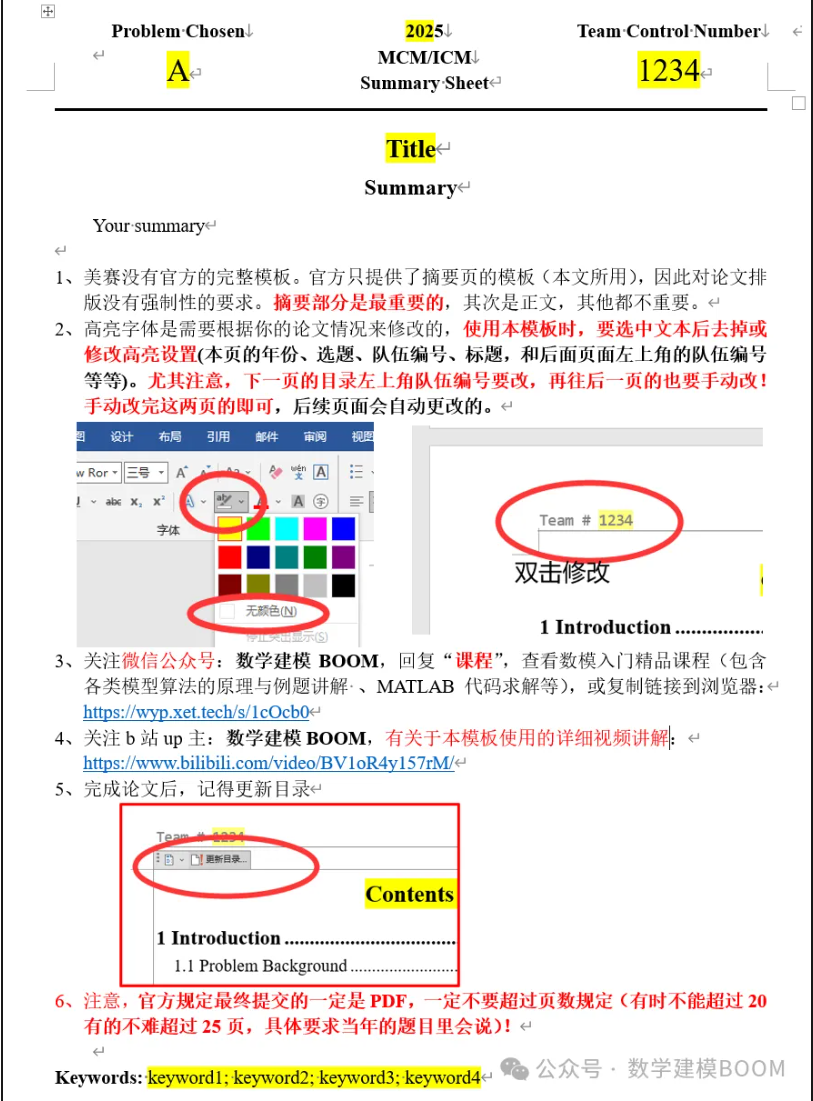
\includegraphics[width=0.8\textwidth]{2}
				\caption{摘要页}
				\label{fig:2}
			\end{figure}
			\begin{itemize}
				\item[$\bullet$] 摘要是竞赛论文的重要组成部分,应作为论文的第一页显示。评委们很看重摘要,获奖论文往往根据摘要的质量与其他论文区别开来。
				\item[$\bullet$] 想要写好摘要,就站在读者的角度想,读了摘要后是否会继续读论文正文;摘要中的精炼描述应当能激发读者继续读下去的兴趣。
				\item[$\bullet$]摘要应该是最后写的,因为摘要需要清楚描述对赛题的解决方法,以及最终求得的结果和结论。确保在所有问题解决后留好充足时间,写一份全面且清晰明了的摘要。 
				\item[$\bullet$] 仅仅复述比赛问题,或者从简介里复制内容作为摘要通常被认为是很菜的
				\item[$\bullet$] 每一小问,都要给一个明确的结果(数值或文字描述)
			\end{itemize}
			$$w < w_0$$
			``Please press the `x' bottom.''
			``Hello.''
			\begin{center}
			练习三线图 \\
			\begin{tabular}{cc}
				\toprule[1.5pt]
				\makebox[0.3\textwidth][c]{符号} & \makebox[0.4\textwidth][c]{意义} \\
				\midrule[1pt]
				$ w $	& 第一个小时内总成本	\\
				$ w_1 $	& 第二个小时内总成本	\\
				\bottomrule[1.5pt]
			\end{tabular}
			\end{center}
			
			\begin{center}
				练习表格 \\
				\begin{tabular}{|l|c|c|c|p{3cm}|}
					\hline
					姓名 & 语文 & 数学 & 外语 & 备注 \\
					\hline
					张三 & 84 & 54 & 55 & 补考另行通知 \\
					\hline
					王五 & 100 & 99 &89 & 优秀 \\
					\hline
				\end{tabular} 
			\end{center}
			
			\begin{center}
				长公式拆行
				\begin{multline}
					a + b + c + d + e + f
					+ g + h + i \\
					= j + k + l + m + n\\
					= o + p + q + r + s\\
					= t + u + v + x + z
				\end{multline}
				多行公式
				\begin{align}
					a & = b + c \notag \\
					& = d + e
				\end{align}
				多行公式进阶
				\begin{align}
					a ={} & b + c \\
					={} & d + e + f + g + h + i + j + k + l \notag \\
					& + m + n + o \\
					={} & p + q + r + s
				\end{align}
				多组公式
				\begin{align}
					a &=1 & b &=2 & c &=3 \\
					d &=-1 & e &=-2 & f &=-5
				\end{align}
			\end{center}
			
			
				
				
				
				
			
\end{document}
